\documentclass[twocolumn]{IEEEtran}
\usepackage{graphicx}
\usepackage[utf8x]{inputenc}
\usepackage{times}
\usepackage{amssymb,amsfonts}
\usepackage[tbtags]{amsmath}
\usepackage{cite}
\usepackage{slashbox}
\usepackage{pict2e}
\usepackage{float}
\usepackage[all]{xy}
\usepackage{graphics,graphicx,color,colortbl}
\usepackage{times}
\usepackage{subfigure}
\usepackage{wrapfig}
\usepackage{multicol}
\usepackage{cite}
\usepackage{url}
\usepackage[tbtags]{amsmath}
\usepackage{amsmath,amssymb,amsfonts,amsbsy}
\usepackage{bm}
\usepackage{algorithm}
\usepackage{algorithmic}
\usepackage[centerlast, small]{caption}
\usepackage[colorlinks=true, citecolor=blue, linkcolor=blue, urlcolor=blue,
breaklinks=true]{hyperref}

\begin{document}
\title{Respuesta transitoria de circuitos de $1^{er}$ y $2^{do}$ orden}
\author{José Fabio Lozano Ovalle Código: $222982$\\
	Wilson Orlando Macias Fuquen Código: $223101$\\
	David Ricardo Martínez Hernández Código: $261931$}
\maketitle
\markboth{Universidad Nacional de Colombia}{}
\floatname{algorithm}{Algoritmo}

\begin{abstract}
.
\end{abstract}

\begin{keywords}
Amortiguamiento crítico, Carga Inicial, Condensador, Constante de Tiempo, Disipación, Energía, Inductor, Subamortiguado, Sobreamortiguamiento, Voltaje Inicial.
\end{keywords}

\section{Objetivos}

\section{Introducción}

\section{Marco Teórico}
\subsection{Circuitos de Primer Orden}
\noindent
Un circuito de \textbf{primer orden} es caracterizado por una ecuación diferencial de primer orden. Existen dos tipos de circuitos que describen este comportamiento, el circuito $RL$ y el $RC$, hay dos formas de excitar el circuito. La primera forma es con las condiciones iniciales de almacenamiento, también llamado circuitos sin fuente (\textit{Source-free Circuits}), asumiendo esa energía inicial de almacenamiento en los elementos inductivos y capacitivos. La energía causa un flujo de corriente en el circuito y es disipada gradualmente en la resistencia\footnote{Texto tomado de \cite{sadiku}, Página 238}.

\subsubsection{Circuitos RC sin fuente}
\noindent
Cuando la fuente DC fue desconectada de repente. La energía almacenada en el condensador es liberada a la resistencia, es decir disipada por dicho elemento.
\begin{figure}[H]
	\centering
		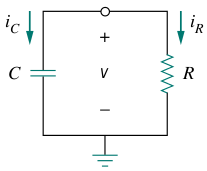
\includegraphics[scale=0.7]{rcsinsource.png}
	\caption{Circuito RC sin fuente. (Tomado de \cite{sadiku}, página 238)}
	\label{rcsin}
\end{figure}
\noindent
En el tiempo $t=0$ el voltaje inicial es
\begin{equation}
 v(0)=V_{0}
\end{equation}
\begin{equation}
 w(0) = \frac{1}{2} C {V_{0}}^{2}
\end{equation}
\noindent
Aplicando Ley de corrientes de Kirchhoff en el nodo de la Fig. \ref{rcsin}
\begin{equation}
 i_C + i_R = 0
\end{equation}
\noindent
Por definición $C\frac{{dv}}{{dt}}$ $\frac{v}{R}$
\begin{equation}
 C\frac{{dv}}{{dt}} + \frac{v}{R} = 0
\end{equation}
\noindent
Al realizar el análisis matemático correspondiente se obtiene la siguiente ecuación diferencial de primer orden
\begin{equation}
 \frac{dv}{v} = -\frac{1}{RC} dt
\end{equation}
\noindent
Obteniendo Al integrar a ambos lados de la ecuación y despejando $v(0)$ se obtiene
\begin{equation}
 v(t) = A{e^{ - t/RC}}
\end{equation}
\noindent
Donde $v(0) = A = V_{0}$, entonces
\begin{equation}
 v(t) = V_{0}{e^{ - t/RC}}
\label{eqnat}
\end{equation}
\noindent
Esta función hace referencia a la respuesta del circuito como una función exponencial decreciente de un voltaje inicial. Cuando no existe una fuente de voltaje o de corriente externa conectada al circuito es llamada la \textit{Respuesta natural del circuito}.
\begin{figure}[H]
	\centering
		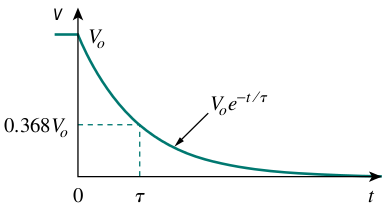
\includegraphics[scale=0.5]{respnat.png}
	\caption{Gráfica de la respuesta natural del circuito RC, de la ecu. (\ref{eqnat}). (Tomado de \cite{sadiku}, página 240)}
	\label{respnat}
\end{figure}
\noindent
Donde $\tau = RC$ es la constante de tiempo, entonces
\begin{equation}
 v(t) = V_{0}{e^{ - t/\tau}}
\label{ecu1}
\end{equation}

\begin{table}[H]
	\centering
\begin{tabular}[c]{|c|c|}\hline
$t$ & $v(t) / V_0$ \\ \hline
$\tau$ & $0.36788$ \\
$2\tau$ & $0.13534$ \\
$3\tau$ & $0.04979$ \\
$4\tau$ & $0.01832$ \\
$5\tau$ & $0.00674$ \\ \hline
\end{tabular}
	\caption{Valores de $v(t) / V_0 = e^{- t / \tau}$. (Tomado de \cite{sadiku}, página 240)}
	\label{tab1}
\end{table}
\noindent
Al conocer el voltaje $v(t)$, se puede encontrar la corriente $i(t)$
\begin{equation}
 i(t) = \frac{v(t)}{R} = \frac{V_0}{R} {e^{ - t/RC}}
\end{equation}
\noindent
La potencia disipada por la resistencia es
\begin{equation}
 p(t)= vi_R= \frac{{V_0}^{2}}{R} {e^{ - 2t/RC}}
\end{equation}
\noindent
La potencia disipada por la resistencia en un tiempo $t$ es
\begin{equation}
{w_R}(t) = \int_0^t {pdt}  = \int_0^t {\frac{{{V_0}^2}}{R}{e^{ - 2t/\tau }}} dt
\end{equation}
\begin{equation}
 {w_R}(t) = \frac{1}{2}C{V_0}^2\left( {1 - {e^{ - 2t/\tau }}} \right)
\end{equation}
\noindent
Notese que cuando $t \rightarrow \infty$, $w_R(\infty) \rightarrow \frac{1}{2}C{V_0}^2$, y como $w_C(0)$ es la energía inicial alamacenada en el condensador. Esa misma energía sera disipada posteriormente en la resistencia.

\subsubsection{Circuito RL sin fuente}
\noindent
Considere una conección en serie de una bobina con inductor y una resistencia Fig. \ref{rlsin}, el objetivo es determinar la corriente de respuesta, la cual se asume como corriente $i(t)$ a través del inductor.
\begin{figure}[H]
	\centering
		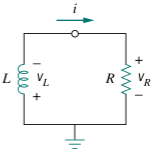
\includegraphics[scale=0.8]{rlsinsource.png}
	\caption{Circuito RL sin fuente. (Tomado de \cite{sadiku}, página 243.)}
	\label{rlsin}
\end{figure}
\noindent
Asumiendo la corriente inicial $I_0$
\begin{equation}
 i(0) = I_0
\end{equation}
\noindent
La correspondiente energía del almacenada en el inductor es
\begin{equation}
 w(0) = \frac{1}{2} L{I_0}^{2}
\end{equation}
\noindent
Aplicando Ley de Voltaje de Kirchhoff en el circuito de la Fig. \ref{rlsin}
\begin{equation}
v_L + v_R = 0 
\end{equation}
\noindent
pero $v_L = L \frac{di}{dt}$ y $v_R = iR$
\begin{equation}
 L \frac{di}{dt} + iR = 0
\end{equation}
\noindent
Al realizar el análisis matemático correspondiente se obtiene la siguiente ecuación diferencial de primer orden
\begin{equation}
 \frac{di}{dt}= - iRL
\end{equation}
\noindent
Obteniendo Al integrar a ambos lados de la ecuación y despejando $i(0)$ se obtiene
\begin{equation}
 i(t) = I_{0}{e^{ - tR/L}}
\label{eqnatrl}
\end{equation}
\noindent
Esta función hace referencia a la respuesta del circuito como una función exponencial decreciente de una corriente inicial.
\begin{figure}[H]
	\centering
		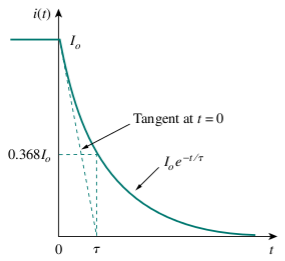
\includegraphics[scale=0.6]{respnatrl.png}
	\caption{Gráfica de la respuesta natural del circuito RL, de la ecu. (\ref{eqnatrl}). (Tomado de \cite{sadiku}, página 244)}
	\label{respnatrl}
\end{figure}
\noindent
Donde $\tau = L/R$ es la constante de tiempo, entonces
\begin{equation}
 i(t) = I_{0}{e^{ - t/\tau}}
\label{ecu2}
\end{equation}
\noindent
Al conocer la corriente $i(t)$, se puede encontrar el voltaje $v(t)$ en la resistencia
\begin{equation}
 v_{R}(t) = i R = I_{0} R {e^{ - t/\tau}}
\end{equation}
\noindent
La potencia disipada por la resistencia es
\begin{equation}
 p=v_{R}i=  {I_{0}}^{2} R {e^{ - 2t/\tau}}
\end{equation}
\noindent
La energía absorbida por la resistencia es
\begin{equation}
 {w_R}(t) = \int_0^t {pdt}  = \int_0^t {{I_0}^2R{e^{ - 2t/\tau }}} dt
\end{equation}
\begin{equation}
 {w_R}(t) = \frac{1}{2}L{I_0}^2\left( {1 - {e^{ - 2t/\tau }}} \right)
\end{equation}
\noindent
Nótese que cuando $t \rightarrow \infty$, $w_R(\infty) \rightarrow \frac{1}{2}L{I_0}^2$, y como $w_L(0)$ es la energía inicial alamacenada en la bobina. Esa misma energía sera disipada posteriormente en la resistencia.

\subsection{Circuitos de Segundo Orden}
\noindent
En los circuitos de primer orden solo se tenían dos elementos, una resistencia con un condensador o una resistencia y una bobina, dichos circuitos tenían una ecuación diferencial de primer orden que describe su comportamiento. Un ejemplo de un circuito de segundo orden es un $RLC$.\\
Un circuito de segundo orden es caracterizado por una ecuación diferencial de segundo orden. Esto consiste en una resistencia y el equivalente de dos elementos de almacenamiento de energía\footnote{Texto tomado de \cite{sadiku}, página 296}.

\subsubsection{Circuitos RLC en serie sin fuente}
\noindent
Un circuito $RLC$ en serie es como la Fig. \ref{rlcserie}, el circuito es inicialmente excitado por la energía almacenada en el condensador y la bobina. La energía es representada por el voltaje inicial en el condensador $V_0$ y la corriente inicial en la bobina $I_0$.
\begin{figure}[H]
	\centering
		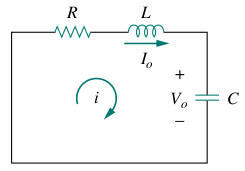
\includegraphics[scale=0.6]{rlcserie.png}
	\caption{Circuito $RLC$ en serie sin fuente. (Tomado de \cite{sadiku}, página 301)}
	\label{rlcserie}
\end{figure}
\begin{equation}
 v\left( 0 \right) = \frac{1}{C}\int_{ - \infty }^0 {idi = {V_0}} 
\end{equation}
\begin{equation}
 i\left( 0 \right) = I_0
\end{equation}
\noindent
Aplicando la ley de de voltajes de Kirchhoff a la Fig. \ref{rlcserie}
\begin{equation}
 R i + L \frac{di}{dt} \frac{1}{C} \int_{ - \infty }^0 {idi = {V_0}} = 0
\end{equation}
\noindent
La ecuación diferencial que se obtiene es
\begin{equation}
 \frac{{{d^2}i}}{{d{t^2}}} + \frac{R}{L}\frac{{di}}{{dt}} + \frac{i}{{LC}} = 0
\label{ecudif2}
\end{equation}
\noindent
El polinomio característico es
\begin{equation}
 s^2 + \frac{R}{L} s + \frac{1}{LC} = 0
\label{polinomio}
\end{equation}
\noindent
Al resolver la ecuación diferencial por algunos de los métodos para la solución de estas ecuaciones. Las raíces que se obtienen son
\begin{equation}
 {s_{1,2}} =  - \frac{R}{{2L}} \pm \sqrt {{{\left( {\frac{R}{{2L}}} \right)}^2} - \frac{1}{{LC}}}
\label{root}
\end{equation}
\begin{equation}
 {s_1} =  - \alpha  + \sqrt {{\alpha ^2} - {\omega _0}^2} \ \ \ \ \ {s_2} =  - \alpha  - \sqrt {{\alpha ^2} - {\omega _0}^2}
\end{equation}
\noindent
Donde
\begin{equation}
 \alpha  = \frac{R}{{2L}}\ \ \ \ \ \ {\omega _0} = \frac{1}{{\sqrt {LC} }}
\end{equation}
\noindent
Las raíces $s_1$ y $s_2$ son llamadas \textit{frecuencias naturales}, esta asociado con la frecuencia natural del circuito, $\omega _0$ es la \textit{frecuencia natural de subamortiguamiento} y $\alpha$ es la \textit{frecuencia neper} o el \textit{Factor de amortiguamiento}. En términos de $\alpha$ y $\omega$ la ecu. (\ref{polinomio})
\begin{equation}
 s^2 + 2 \alpha s + {\omega _0} ^ {2}
\end{equation}
\noindent
La solución a la ecuación diferencial es
\begin{equation}
 i(t) = A_1{e ^{s_1 t}} + A_2{e ^{s_2 t}}
\label{solve}
\end{equation}
\noindent
cuando las constantes $A_1$ y $A_2$ son determinados por las condiciones iniciales por los valores de $i(0)$ y $\frac{di(0)}{dt}$.\\
Para las ecu. (\ref{root}), se pueden encontrar tres tipos de soluciones:
\begin{enumerate}
 \item Si $\alpha > \omega _0$, se tiene un caso de \textit{sobreamortiguamiento}
 \item Si $\alpha = \omega _0$, se tiene un caso de \textit{críticamente amortiguado}
 \item Si $\alpha < \omega _0$, se tiene un caso de \textit{subamortiguamiento}
\end{enumerate}

\subsubsection*{Sobreamortiguamiento $\alpha > \omega _0$}
\noindent
Cuando $C > 4L/{R^2}$, esto determina las raíces $s_1$ y $s_2$ negativas y reales
\begin{equation}
 i(t) = A_1{e ^{s_1 t}} + A_2{e ^{s_2 t}}
\end{equation}
\begin{figure}[H]
	\centering
		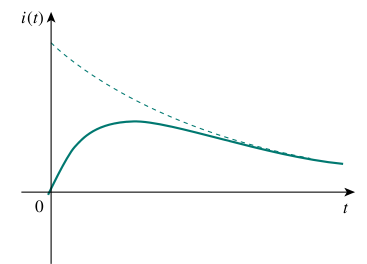
\includegraphics[scale=0.5]{sobre.png}
	\caption{Respuesta a un circuito sobreamortiguado. (Tomado de \cite{sadiku}, página 304)}
	\label{subamortiguado}
\end{figure}

\subsubsection*{Críticamente amortiguado $\alpha = \omega _0$}
\noindent
Cuando $C = 4L/{R^2}$, las raíces $s_1=s_2$ las rices son reales e iguales, la respuesta a la ecuación diferencial es
\begin{equation}
 i(t) = ({A_1} + {A_2}t){e ^{\alpha t}}
\end{equation}
\noindent
la respuesta natural del circuito críticamente amortiguado es una suma de dos términos: un exponencial negativo y un exponencial negativo multiplicado por un término linea
\begin{equation}
 i(t) = ({A_2} + {A_1}t){e ^{-\alpha t}}
\end{equation}
\begin{figure}[H]
	\centering
		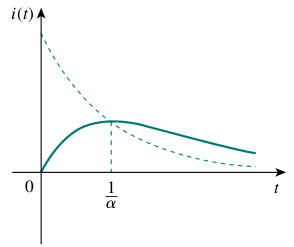
\includegraphics[scale=0.5]{amor.png}
	\caption{Respuesta a un circuito críticamente amortiguado. (Tomado de \cite{sadiku}, página 304)}
	\label{amortiguado}
\end{figure}

\subsubsection*{Subamortiguado $\alpha < \omega _0$}
\noindent
Cuando $C < 4L/{R^2}$ las raíces son complejas conjugadas
\begin{equation}
 {s_1} =  - \alpha  + \sqrt {{\alpha ^2} + {\omega _0}^2}  =  - \alpha  + j{\omega _d}
\end{equation}
\begin{equation}
 {s_2} =  - \alpha  + \sqrt {{\alpha ^2} - {\omega _0}^2}  =  - \alpha  + j{\omega _d}
\end{equation}
\noindent
donde $j=\sqrt{(-1)}$ y $\omega _d = \sqrt {{\alpha ^2} + {\omega _0}^2}$, la cual es llamada \textit{Frecuencia de amortiguamiento}. $\omega _0$ llamada también \textit{frecuencia natural de subamortiguamiento} y $\omega _d$ llamada \textit{frecuencia natural de amortiguamiento}. La respuesta final es
\begin{equation}
 i(t) = {e^{ - \alpha t}}\left( {{C_1}\cos {\omega _d}t + {C_2}\sin {\omega _d}t} \right)
\end{equation}
\noindent
El periodo $T= \frac{2\pi}{\omega _d}$
\begin{figure}[H]
	\centering
		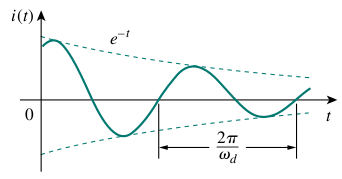
\includegraphics[scale=0.5]{sub.png}
	\caption{Respuesta a un circuito subamortiguado. (Tomado de \cite{sadiku}, página 304)}
	\label{subamortiguado}
\end{figure}

\subsubsection{Circuitos RLC en paralelo sin fuente}
\noindent
Un circuito $RLC$ en paralelo es como Fig. \ref{rlcparalelo}. El análisis es muy similar al anterior. Es inicialmente excitado por la energía almacenada en el condensador y la bobina. La energía es representada por el voltaje inicial en el condensador $V_0$ y la corriente inicial en la bobina $I_0$.
\begin{figure}[H]
	\centering
		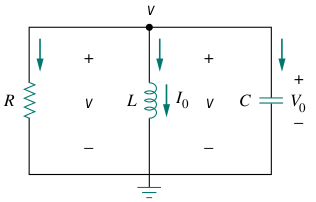
\includegraphics[scale=0.5]{rlcparalelo.png}
	\caption{Circuito RLC en paralelo sin fuente. (Tomado de \cite{sadiku}, página 308)}
	\label{rlcparalelo}
\end{figure}
\begin{equation}
 i\left( 0 \right) = \frac{1}{L}\int_{ - \infty }^0 {vdi = {I_0}} 
\end{equation}
\begin{equation}
 v\left( 0 \right) = V_0
\end{equation}
\noindent
Aplicando la ley de de voltajes de Kirchhoff a la Fig. \ref{rlcparalelo}
\begin{equation}
\frac{v}{R}  + \frac{1}{L}\int_{ - \infty }^0 {vdi = {I_0}} + C\frac{dv}{dt} = 0
\end{equation}
\begin{equation}
 \frac{v}{R} + \frac{1}{{RC}}\frac{{dv}}{{dt}} + \frac{1}{{LC}}v = 0
\end{equation}
\noindent
la ecuación característica que se obtiene es
\begin{equation}
 s^2 + \frac{1}{RC}s +  \frac{1}{LC} = 0
\end{equation}
\noindent
Las raíces del polinomio son
\begin{equation}
 {s_{1,2}} =  - \frac{1}{{2RC}} \pm \sqrt {{{\left( {\frac{1}{{2RC}}} \right)}^2} - \frac{1}{{LC}}} 
\end{equation}
\begin{equation}
 {s_{1,2}} =  - \alpha \pm \sqrt {{{ \alpha ^2} - {\omega _0}^2}} 
\end{equation}
\noindent
donde
\begin{equation}
 \alpha  = \frac{1}{{2RC}}\ \ \ \ \ \ {\omega _0} = \frac{1}{{\sqrt {LC} }}
\end{equation}
\noindent
Los tres tipos de soluciones:
\begin{enumerate}
 \item Si $\alpha > \omega _0$, se tiene un caso de \textit{sobreamortiguamiento}
 \item Si $\alpha = \omega _0$, se tiene un caso de \textit{críticamente amortiguado}
 \item Si $\alpha < \omega _0$, se tiene un caso de \textit{subamortiguamiento}
\end{enumerate}

\subsubsection*{Sobreamortiguamiento $\alpha > \omega _0$}
\noindent
Cuando $L > 4{R^{2} C}$, esto determina las raíces $s_1$ y $s_2$ negativas y reales
\begin{equation}
 v(t) = A_1{e ^{s_1 t}} + A_2{e ^{s_2 t}}
\end{equation}

\subsubsection*{Críticamente amortiguado $\alpha = \omega _0$}
\noindent
Cuando $L = 4{R^{2}C}$, las raíces $s_1=s_2$ las rices son reales e iguales, la respuesta a la ecuación diferencial es
\begin{equation}
 v(t) = ({A_1} + {A_2}t){e ^{-\alpha t}}
\end{equation}

\subsubsection*{Subamortiguado $\alpha < \omega _0$}
\noindent
Cuando $L < 4{R^{2}C}$ las raíces son complejas conjugadas
\begin{equation}
 s_{1,2} = -\alpha \pm i \omega _d
\end{equation}
\noindent
\begin{equation}
 \omega _d = \sqrt {{\omega _0}^2 - {\alpha ^2}}
\end{equation}
\noindent
La respuesta final del circuito sera
\begin{equation}
 v(t) = {e^{ - \alpha t}}\left( {{C_1}\cos {\omega _d}t + {C_2}\sin {\omega _d}t} \right)
\end{equation}
\noindent
Las constantes $A_1$ y $A_2$ son determinadas por las condiciones iniciales

\section{Materiales}
\begin{itemize}
 \item .
 \item .
 \item .
 \item .
 \item .
 \item .
\end{itemize}

\section{Análisis y Resultados Teóricos}

\section{Preguntas}

\bibliographystyle{ieeetran}
\begin{thebibliography}{99}
\bibitem{dorf} Dorf  \& Svoboda.
{\em "`Circuitos Eléctricos"'}.
Alfaomega, Sexta Edición, 2006.

\bibitem{sadiku} Alexander, Charles K. \&  Sadiku, Matthew N.O.
{\em "`Fundamentals of Electric Circuits"'}.
McGRAW-HILL, ISE Editions, 1999.

\bibitem{nahvi} Nahvi, Mahmood \& Edminister, Joseph A.
{\em "`Theory and Problems of Electric Circuits"'}.
McGRAW-HILL, Fourth Edition, 2003.
\end{thebibliography}
\end{document}
